%!TEX root = ../memoire.tex

\chapter{Génération automatique de texte}

La génération automatique de texte découle de la branche qu'est le \ac{TAL}. Reiter et Dale \citep{ReiterBuildingNaturalLanguage2000} définissent cette branche comme étant un domaine à la croisée des chemins entre l'intelligence artificielle et la linguistique computationnelle. L'objectif est de développer des sytèmes pouvant produire du texte compréhensible en langue naturelle à partir de données non-linguistiques. Bien que l'objectif est commun à tous ces systèmes, les moyens pour s'y rendre sont de divers ordres. Entre autre car il existe des inputs de diverses natures : données, texte et images(Thomason et al., 2014). Ensuite car il y existe diverses approches de réalisation de texte : templates, règles, stochastiques \citep{gatt18}.

Toutefois, avant d'entrer dans les détails de la \ac{GAT}, il serait intéressant de mentionner l'origine de ces systèmes. À la base, ils ont été conçus pour, entre autre, générer des rapports automatiquement afin de faciliter le travail des humains. Effectivement, il est très utile pour certains de pouvoir lire un résumé de données numériques analysées par un système informatique. Tel que JSreal le mentionne, avec la GAT on peut présenter un résumé d'information provenant d'input numérique qui serait incompréhensible, mais utile pour un humain qui n'est pas un expert, et donc incapable de déchiffrer ces données. En plus d'être capable de résumé ces informations, le système informatique a l'avantage de fournir ces rapports sans se fatiguer à faire une tâche extrêmement monotone, qui pourrait être très coûteuse en termes de temps et de ressources pour des être humains.  D'ailleurs, pour qu'ils soient utiles, les textes générés automatiquement n'ont pas besoin d'être lus par une quantité phénomènale de gens. Dès qu'ils remplissent leur fonction, en étant utile à ne serait-ce que quelques personnes, leur raison d'être sera justifiée.  Dans cette même optique, il s'est développé des systèmes pouvant générer du texte en fonction de l'utilisateur. Ainsi, on pourrait générer un rapport X en fonction du professionnel, du technicien ou du client (Mahammood Reiter,2011) qui lira ce texte. Cette utilisation de la \ac{GAT} s'applique à de nombreux domaines dont les textes journalistiques. Les articles décrivant les matchs sportifs qui ne bénéficient pas de couverture médiatique (Van der Lee, 2017) sont des applications concrètes et utile du développement en \ac{GAT}. De même que des rapports générés automatiquement sur la qualité de l'air en fonction de l'utilisateur \citep{WannerMARQUISGENERATIONUSERTAILORED2010}. Ainsi, via le développement de ces systèmes, l'effacité des ordinateurs et de l'accessibilité aux données grandissante, on est capable de générer un article de journal automatiquement suivant les minutes où un évènement se produit(Oremus,2014). On parle là de robo-journalisme à son plein essor.

De nos jours la \ac{GAT} a grandement changé depuis que Dale et Reiter ont publié leur livre. Bien que ce soit le livre le plus complet entourant la NLG, le domaine a changé avec l'émergence de text-to-text generation et de vision-to-text generation(Hendricks et al., 2016a). qui reposent plus sur des méthodes statistiques que les modèles traditionnels de data-to-text qui étaient rule-based ou template based \citep{gatt18}. D'ailleurs, les frontières entre les diverses approches s'affaissent aussi avec le temps et nous sommes témoins d'une apparition constante de systèmes hybrides. Par exemple, des systèmes à base de patrons utilisant des règles de grammaire, des systèmes à base de règles utilisant des méthodes statistiques pour combler certaines tâches \citep{gatt18}. C'est donc un domaine très vaste qui, à ce jour, n'est pas uniforme. Ce qui est directement lié à une grande variété en NLG: divers types d'input (type de données), divers objectifs (tâches), diverses approches. Il est aussi important de préciser que la \ac{GAT} a aussi une valeur linguistique théorique. Il existe des linguistes qui testent leur théories via le développement de générateur automatique de texte. C'est effectivement une bonne manière de vérifier si un modèle théorique fonctionne\citep{DanlosPresentationmodelegeneration1983}. 

Dans le cadre de ce mémoire, notre projet est un réalisateur. La réalisation linguistique étant une étape du processus entourant la \ac{GAT}, nous ne travaillons que sur celle-ci. D'ailleurs notre réalisateur est créé avec des perspectives linguistiques. Ce qui exclut les systèmes à base de patrons et les systèmes statistiques, car ceux-ci ne nécessitent pas d'analyse linguistique pour le bon fonctionnement de la réalisation. Notre système se base sur des règles grammaticales. Cependant, avant de décrire notre projet, nous allons jeter les bases de la \ac{GAT} en décrivant le pipeline classique et en exposant quelques réalisateurs linguistiques.

\section{Pipeline classique GAT}

À la base, le pipeline classique observé par Dale et Reiter est un processus séquentiel séparé en diverses sections \citep{ReiterBuildingNaturalLanguage2000}. Traditionnellement, les six étapes suivantes sont les plus utilisées selon Dale et Reiter, comme illustré à la figure~\ref{fig:Pipeline}.
%les figures latex bougent, donc évite les formulations comme ça.
\begin{figure}[htb] % utilise toujours [htb]
	\centering
	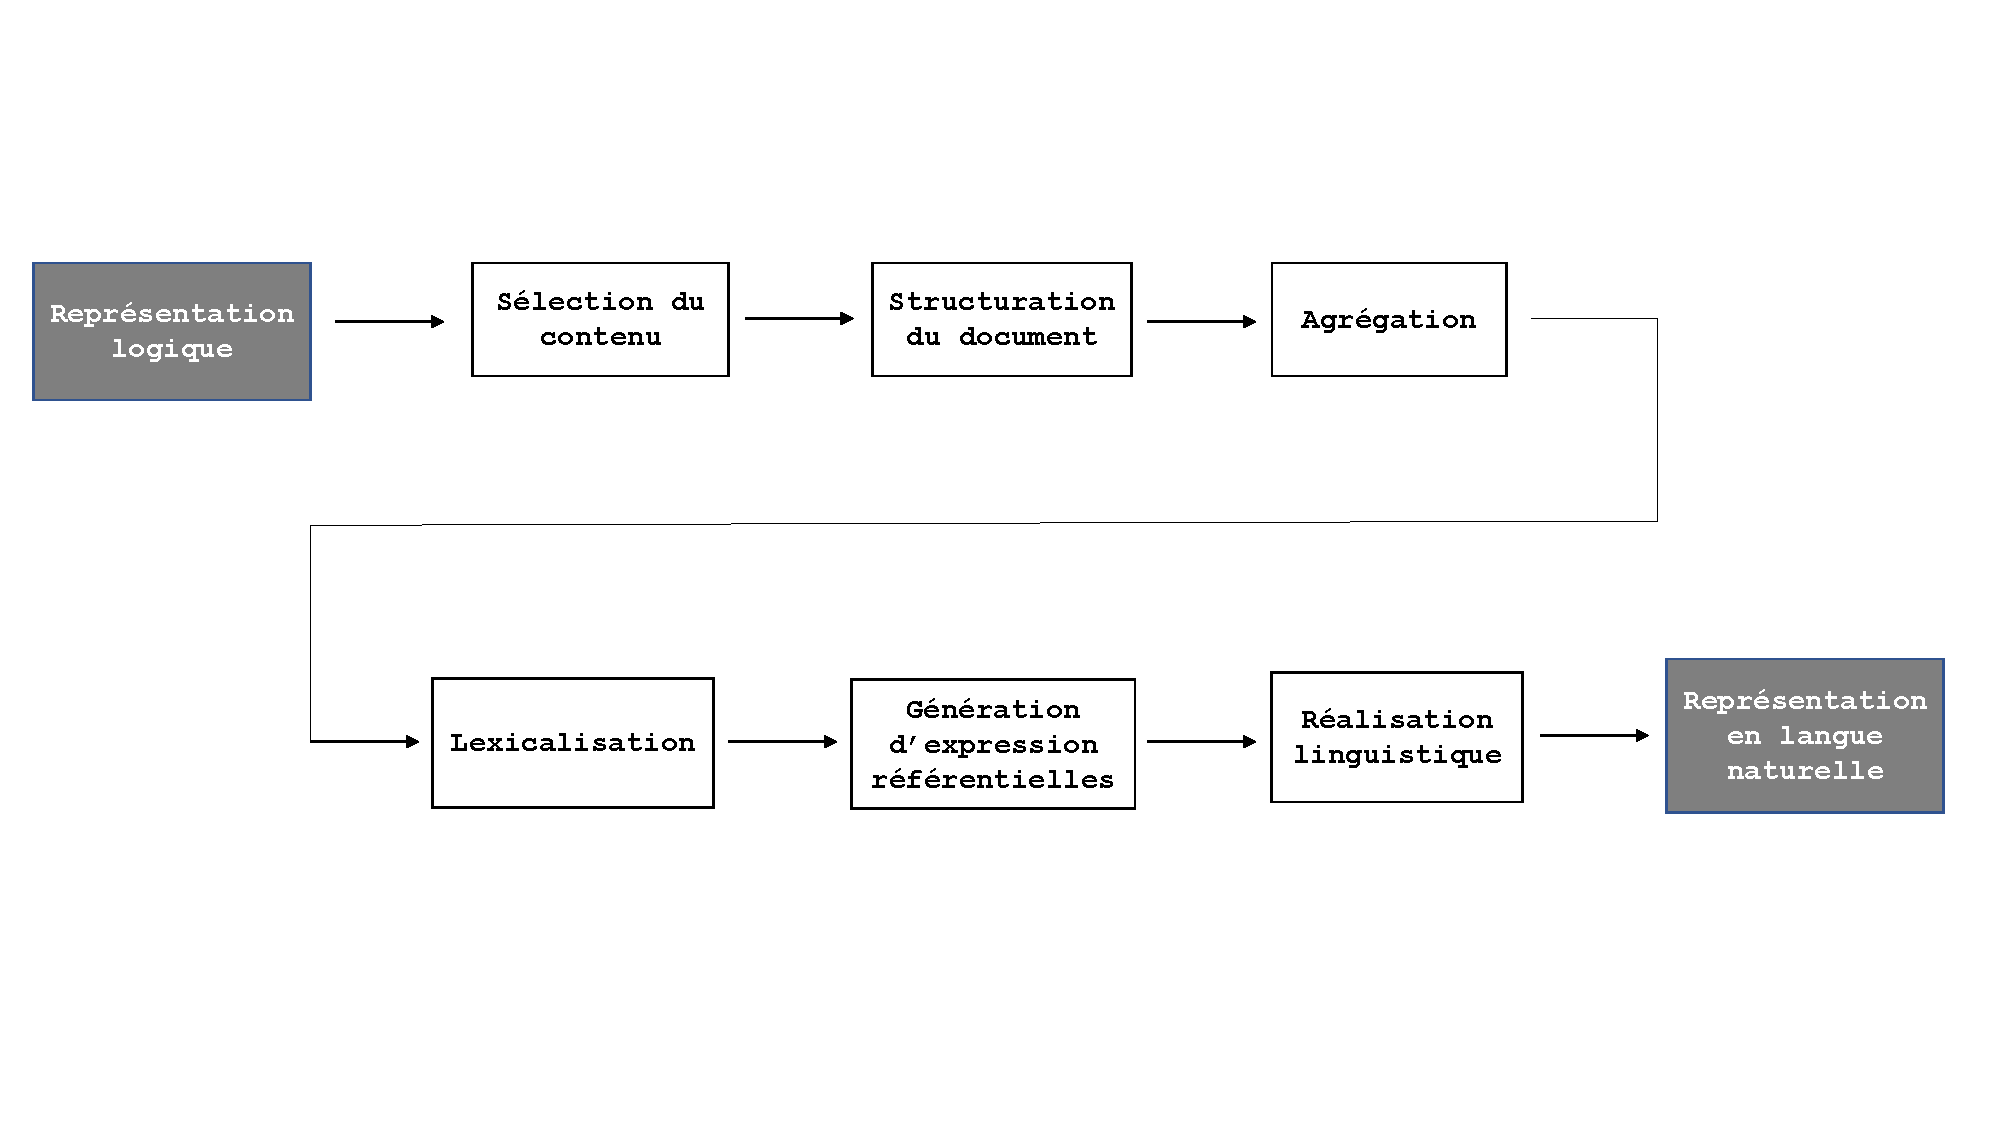
\includegraphics[width=1\textwidth, trim = {0cm 0cm 0cm 0cm},clip]{ch2/figs/pipeline.pdf}
	\caption{Pipeline classique}
	\label{fig:Pipeline}
\end{figure}

\draft{Beaucoup s'entendent pour dire qu'il y a deux parties. Le \emph{quoi-dire} et le \emph{comment-le-dire} selon \citep{DanlosPresentationmodelegeneration1983}, puis le \emph{early process} et le \emph{late process}  selon \citep{gatt18}. Le quoi-dire (\emph{early process}) fait référence à blablabla et le comment-le-dire (\emph{late process}) fait référence à blabla.}

\subsection{Sélection du contenu}

Un système de \ac{GAT} doit sélectionner quelles informations seront inclues dans le texte en construction et quelles informations n'y seront pas. La sélection du texte dépend entre autre de l'objectif de la tâche (par exemple si un texte est adressé à un débutant ou un expert), ainsi typiquement , il y a plus d'information ou de détails dans les données que d'information que nous voulons transmettre en texte. Ainsi, la sélection de contenu implique des choix. Par exemple, s'il s'agit de données pour un match de soccer, on ne voudrait probablement pas réaliser toutes les passes et les fautes commises durant le match, bien que ces informations figurent dans les données en input. Il faut donc les filtrer et créer des représentations sémantiques de l'information qui sont souvent exprimé en représentation formelle du langage comme des représentations logiques, des base de données, des matrices ou des graphes.

\subsection{Structuration du document}
Après avoir sélectionné le contenu, un système NLG doit décider l'ordre dans lequel les informations seront présentées. Par exemple, si on utilise encore l'exemple du soccer, on commencerait par les informations générales liées au match (où et quand le match a eu lieu, entre quelles équipes, qui était blessé cette journée, etc), puis la description des buts comptés en ordre chronologique. Ce qui résulte de cette étape du processus est le plan d'un texte: une représentation ordonnée et structurée de messages à transmettre. Durant les dernières années, il y a eu des tentatives d'implémenter des méthodes d'apprentissage machine pour que la structuration de document se fasse automatiquement (Dimitromanolaki et Androutsopoulos,2003; Althaus et al., 2004)

\subsection{Agrégation}
Ce ne sont pas tous les messages sélectionnés dans le plan qui doivent être exprimés dans des phrases individuelles. En combinant des phrases individuelles en une seule et même phrase, on génère un texte beaucoup plus fluide et agréable à lire (Cheng et Mellish, 2000). Ainsi, la majeure partie du temps, elle sert à enlever la redondance dans le texte. Encore une fois, des chercheurs tentent d'automatiser cette étape en implémentant des méthodes d'apprentissage machine pour que le système NLG apprenne les règles d'agrégation et les applique lorsqu'il se doit (Barzilay et Lapata, 2006).

\subsection{Lexicalisation}
À cette étape, nous avons des données sélectionnées, puis structurées et que les futures phrases ont été combinées, on peut commencer à traduire les données en langue naturelle. Cette partie est très importante car c'est là qu'on choisi les mots qui seront utilisés pour transmettre le message. Toutefois, cette section se complique parfois car il existe naturellement plusieurs manières différentes de dire la même chose. La complexité de ce processus de lexicalisation dépend des mécanismes intégrés au système pour gérer cela. Certains traitent de lexicalisation en surface, d'autres la traite profondément. Toutefois, ceux qui traitent la lexicalisation en surface sont beaucoup plus restreints dans leur choix et sont très rigides. Tandis qu'un modèle profond permet de mieux tenir compte de la richesse lexicale d'une langue, mais il faudra une approche qui unit les représentations conceptuelles avec des règles de grammaire qui encoderont les choix lexicaux et syntaxiques. D'ailleurs, (Elhadad et al. 1997) avait grandement contribué pour cela.

Convertir un graphe sémantique d'entités et de relations, en un graphe syntaxique de mots et de relations syntaxiques. 

\subsection{Génération d'expressions réferentielles}
Souvent référée comme étape discriminatoire dont le but est de déterminer quelles informations doivent être générées pour qu'on puisse distinguer toutes les entités en jeu. Le but est de s'assurer que le lecteur peut idientifier chaque entité dans le texte. La meilleure manière de référer à une entité donnée.
Il s'agit de la tâche pour sélectionner des mots ou des phrases qui identifieront des entités. C'est une étape du processus qui a reçu beaucoup d'attention, car il n'y a toujours pas de consensus quant à la manière de faire et c'est extrêmement difficle. (Compléter avec les autres articles)

\subsection{Réalisation linguistique}
La dernière étape de ce pipeline NLG classique est la réalisation linguistique. Lorsque tous les mots, puis successivement les phrases ont été choisies, il faut les combiner en des phrases grammaticales. Cette tâche implique couramment l'application de traits morpho-syntaxiques et la linéarisation. De même qu'insérer les mots fonctionnels (auxiliaires, etc.) et la ponctuation. (Lambrey,2016) Objectif: appliquer règles et procédés d'ordre grammaticaux aux représentations abstraites pour que l'output satisfasse les contraintes syntaxiques et morphologiques de la langue en question.

\subsubsection{À base de patrons}
Est utilisé lorsque le domaine est petit et que les variations sont minimes. (McRoy et al., 2003). Montrer un exemple avec le soccer. (p.19).  L'avantage d'utiliser les templates est qu'on peut très bien prévoir ce qui sera généré en output, donc les risques d'erreurs grammaticales sont extrêmement faibles, du au contrôle qu'on a. Ils peuvent aussi être complémenter par des modules de règles pour pallier à certains problèmes, ce qui les rend très performant. Toutefois, l'inconvénient de tels systèmes est qu'ils sont très coûteux en termes de temps, puisque tout doit être fait à la main. Bien qu'avec la mode de l'apprentissage machine, certains systèmes apprennent à écrire des patrons (Angeli et al., 2012). Finalement, ils ne fonctionnent pas bien avec des tâches qui requièrent beaucoup de variation linguistique.

\subsubsection{À base de règles grammaticales}
en parler brièvement

\subsubsection{Statistique}

en parler brièvement et nommer quelques systèmes
mentionner que c'est à la mode


\subsubsection{Règles vs statistiques : avantages/inconvénients}
(Belz et Kow, 2009) et (Vicente et Al., 2015)
Depuis le début de cette section, nous disons qu'il y existe les méthodes staitsitques, et bcp vantent leur mérite, mais certains se sont penchés pour voir jusqu'à quel point ils sont bons. Dans cette partie, parler du blog de E.Reiter et l'article de Belz (si le temps, l'article de Vicente)

\draft{Mentionner le blog de E.Reiter concernant les approches ML et la NLG (rule-based est meilleur, mais on pourrait se servir de ML, sans toutefois rely dessus à 100\% comme certains chercheurs le font.
source (\url{https://ehudreiter.com/2016/12/12/nlg-and-ml})}

\section{Réalisation}

Tel qu'explicité dans le tableau~\ref{fig:Pipeline}, la réalisation est la dernière étape dans le processus de \ac{GAT}. Toutefois, pour beaucoup de chercheurs, elle ne représente pas toujours les tâches décrites précédemment. Il règne une ambiguité quant aux concepts qu'incarne la réalisation. Lambrey le mentionne \citep{LambreyImplementationcollocationspour2017} dans son mémoire, effectivement, \emph{réalisation} peut faire référence aux engins qui font la tâche de réalisation linguistique telle que décrite par le pipeline classique, mais elle réfère aussi aux engins qui englobent l'ensemble des tâches du module de réalisation linguistique. Pour effectuer celles-ci, ces engins partent d'un niveau plus abstrait que la réalisation dans le pipeline classique. C'est pourquoi nous faisons une distinction entre réalisateur de surface et réalisateur profond.Comme le mentionne aussi Dale et Essers 1998 \citep{EssersChoosingSurfaceRealiser1998}, puisque le pipeline est très long à construire en NLG, il n'est pas rare que des gens construisent leur système de NLG comme bon leur semble, mais qu'ils utilisent des réalisateurs déjà existant sur le marché. :The task of building a complete natural language generation nlg system is difficult and complex. Rather than start from scratch, it makes sense to make use of whatever reusable components are available, just as someone building a complete natural language analysis system would be likely to make use of an existing parser for syntactic analysis. In the context of nlg the state of the art is such that a number of reusable components are available for that subtask in the nlg process generally referred to as linguistic realisation.\draft{comment mettre une citation en LaTex : Comme Lavoie le mentionne \citep{LavoieFastPortableRealizer1997} : It is in the realizer that knowledge about the target language resides (syntax, morphology, idiosyncratic properties of lexical items). La nécessité de créer des réalisateurs provient du fait que Realization is fairly well understood both from a linguistic and from a computational point of view, and therefore most projects that use text generation do not include the realizer in the scope of their research.Instead, such projects use an off-the-shelf realizer like Surge.}

Polguère \citep{PolguerePourmodelestratifie} parle des différents modèles de GAT.

\subsection{Réalisateurs de surface}

Les réalisateurs de surface sont appelés ainsi car ils partent d'une représentation syntaxique et lexicalisée, donc peu abstraite en comparaison avec les réalisateurs profonds. Ils correspondent plus à la phase de réalisation linguistique classique mentionnée dans le pipeline classique de Dale et Reiter. Dans le sens où ils s'occupent de blablabla.

\subsubsection{SimpleNLG}
 \citep{GattSimpleNLGRealisationEngine2009}
Dans les années passés, un consensus s'est fait autour de la tâche de réalisation via RealPro, KPML, Surge. La réalisation implique deux tâches logiquement distinctes. La première est faire les bons choix linguisitques compte tenu de l'input sémantique donné. Puis une fois que c'est fait, construire la représentation syntaxique, faire la morphologie et linéariser les phrases sont des opérations assez mécaniques. Ainsi, Simple NLG est un engin de réalisation qui s'occupe des tâches plus mécaniques. Son rôle est de résumer un large volume de données numériques. Processus de réalisation : couvrir la syntaxe et la morphologie anglaise et la linéarisation. Simple NLG c'est une bibliothèque Java, qui fournit des interfaces offrant un contrôle direct sur le processus de réalisation (comment les phrases sont construites, fléchies, combinées et linéarisées).

Ce que SimpleNLG fait: défins un ensemble de types lexicaux et phrastiques correspondant aux catégories grammaticales majeures, il décrit aussi les manières de les combiner. SimpleNLG prend en entrée des constituants simples ou des morceaux de phrases préfabriquées.

Pour construire la structure syntaxique et la linéraiser, il faut faire les quatre étapes suivantes :
Premièrement, initilaiser les constitutants de base avec leurs unités lexicales correspondantes, deuxièmement déterminer les trais lexicaux des unités, troisièmement combiner les constituents en de plus grandes structures syntaxiques et quatrièmement, passer les structures résultantes au linéarisateur qui s'occupe de la linérisation et de mettre les formes fléchies aux unités lexicales en fonction des règles morphologiques.

Ainsi, il y existe un module lexical et un module syntaxique. Le module lexical comprend : le dictionnaire comme tel qui contient les unités lexicale, leur appartenance à une catégorie grammaticale, leurs propriétés syntaxiques et morphologiques. Le module syntaxique décrit les phénomènes morpho-syntaxiques et les règles qui permettent de créer des syntagmes jusqu'à créer une structure syntaxique complète d'un énoncé. Il se veut aussi un réaliseur facile d'utilisation, tel que son nom l'indique \citep{DaoustJSREALTextRealizer2015}.

Noter que SimpleNLG a été traduit dans plusieurs langues : espagnol, italien, et français, portugais (Mazzei et al., 2016, Ramos-Soto 2017, Vaudry ;Lapalme 2013 ; Oliveira et Sripada)

\subsubsection{JSreal} \citep{DaoustJSREALTextRealizer2015}

JSreal qui est en fait JavaScript Realiser. C'est un réaliseur de texte orienté pour les programmeurs web. C'est un réaliseur de texte en français qui génère des expressions et phrases bien formées qui elles peuvent être formattées en HTML pour être explosé dans un browser. Il peut aussi s'employer seul à des fins purement linguistiques ou être intégéré dans des générateurs de textes. Les Specs de JSreal sont similaires à ceux de SimpleNLG.

Pour générer du texte JSreal prend en input des arbres syntaxiques (écrits en java), qui seront ensuite parser en un arbre syntaxique, qui sera par la suite linéarisé. Pour générer du texte, JSreal possède les modules suivants : un lexicon, en ensemble de règles syntaxiques et un ensemble de règles morphologiques. Son dictionnaire défini la catégorie des mots qui le peuple, et les traits (genre, nombre, irrégularités, etc.). Les règles morphologiques : permet d'utiliser les bonnes formes fléchies. Les règles syntaxiques 

Florie ": JSreal prend en entrée des spécifications d'arbres syntaxiques en constituants immédiats écrites en fonctions JavaScript (JS). Les mots, syntagmes, etc. sont les « unités » manipulées. Les unités de base sont les catégories grammaticales (nom, verbe, etc.). Chacune déclenche l'application d'une fonction prenant un lemme comme argument et retournant un objet JS avec les propriétés et méthodes correspondants. Les syntagmes sont des unités déclenchant des fonctions prenant d'autres unités comme arguments. Les lemmes et leurs caractéristiques (traits sont répertoriés dans un dictionnaire à part. L'application des fonctions permet de construire une structure de données sous forme d'arbre regroupant toutes les propriétés des lemmes. Cet arbre est ensuite parcouru et fournit la liste des tokens de la phrase finale."

Mentionner qu'il existe aussi une version bilingue de JSreal \citep{MolinsJSrealBBilingualText2015}

\subsection{Réalisateurs profonds}

Ce qui caractérise les réalisateurs profonds : nécessite un théorie sous-jacente pour traiter les phénomènes, traitent l'interface sémantique-syntaxe,

\subsubsection{RealPro}
\citep{LavoieFastPortableRealizer1997}
RealPro est implémenté en C++, il peut donc se transposer à d'autres plateformes. Il prend en input des arbres de dépendances. Les connaissances syntaxiques et lexicales sont encodées dans un fichier ASCII, ce qui leur permet d'être mis-à-jour. Donc, il prend en input des strctures syntaxiques profondes, inspiré de la TST(melcuk). Les noeuds des arbres syntaxiques sont déjà lexicalisés, ce qui fait que ce système part d'une arbre syntaxique déjà lexicalisé et non d'un input sémantique. Les arcs qui lient les noeuds entre eux sont étiquettées par des relations syntaxiques. Ainsi, RealPro ne fait pas l'étape du choix lexical, donc la réalisation se fait à partir d'unités déjà lexicalisées. Ils ont préféré laisser la lexicalisation à un autre module. L'architecture de RealPro est basé sur la TST. Séquence de correspondance entre différents niveaux de représentations. Ainsi, pour passer de la structure profonde à la strucutre de surface, le logiciel vérifie dans son dictionnaire et ses règles de grammaires pour s'assurer que le passage à la seconde représentation syntaxique est correcte. Son linguistic Knowledge Base est réparti en divers modules dont  le lexique, les règles de grammaires. Ceux-ci seront réquisitionnés par les diverses composantes qui composent le pipeline de ce système. Voici en ordre, les composantes les plus importantes : Deep-syntactic component, Surface syntactic component, Deep-morphological component.

Voici un graphique représentant le pipeline de ce système :
\begin{figure}[h]
	\centering
	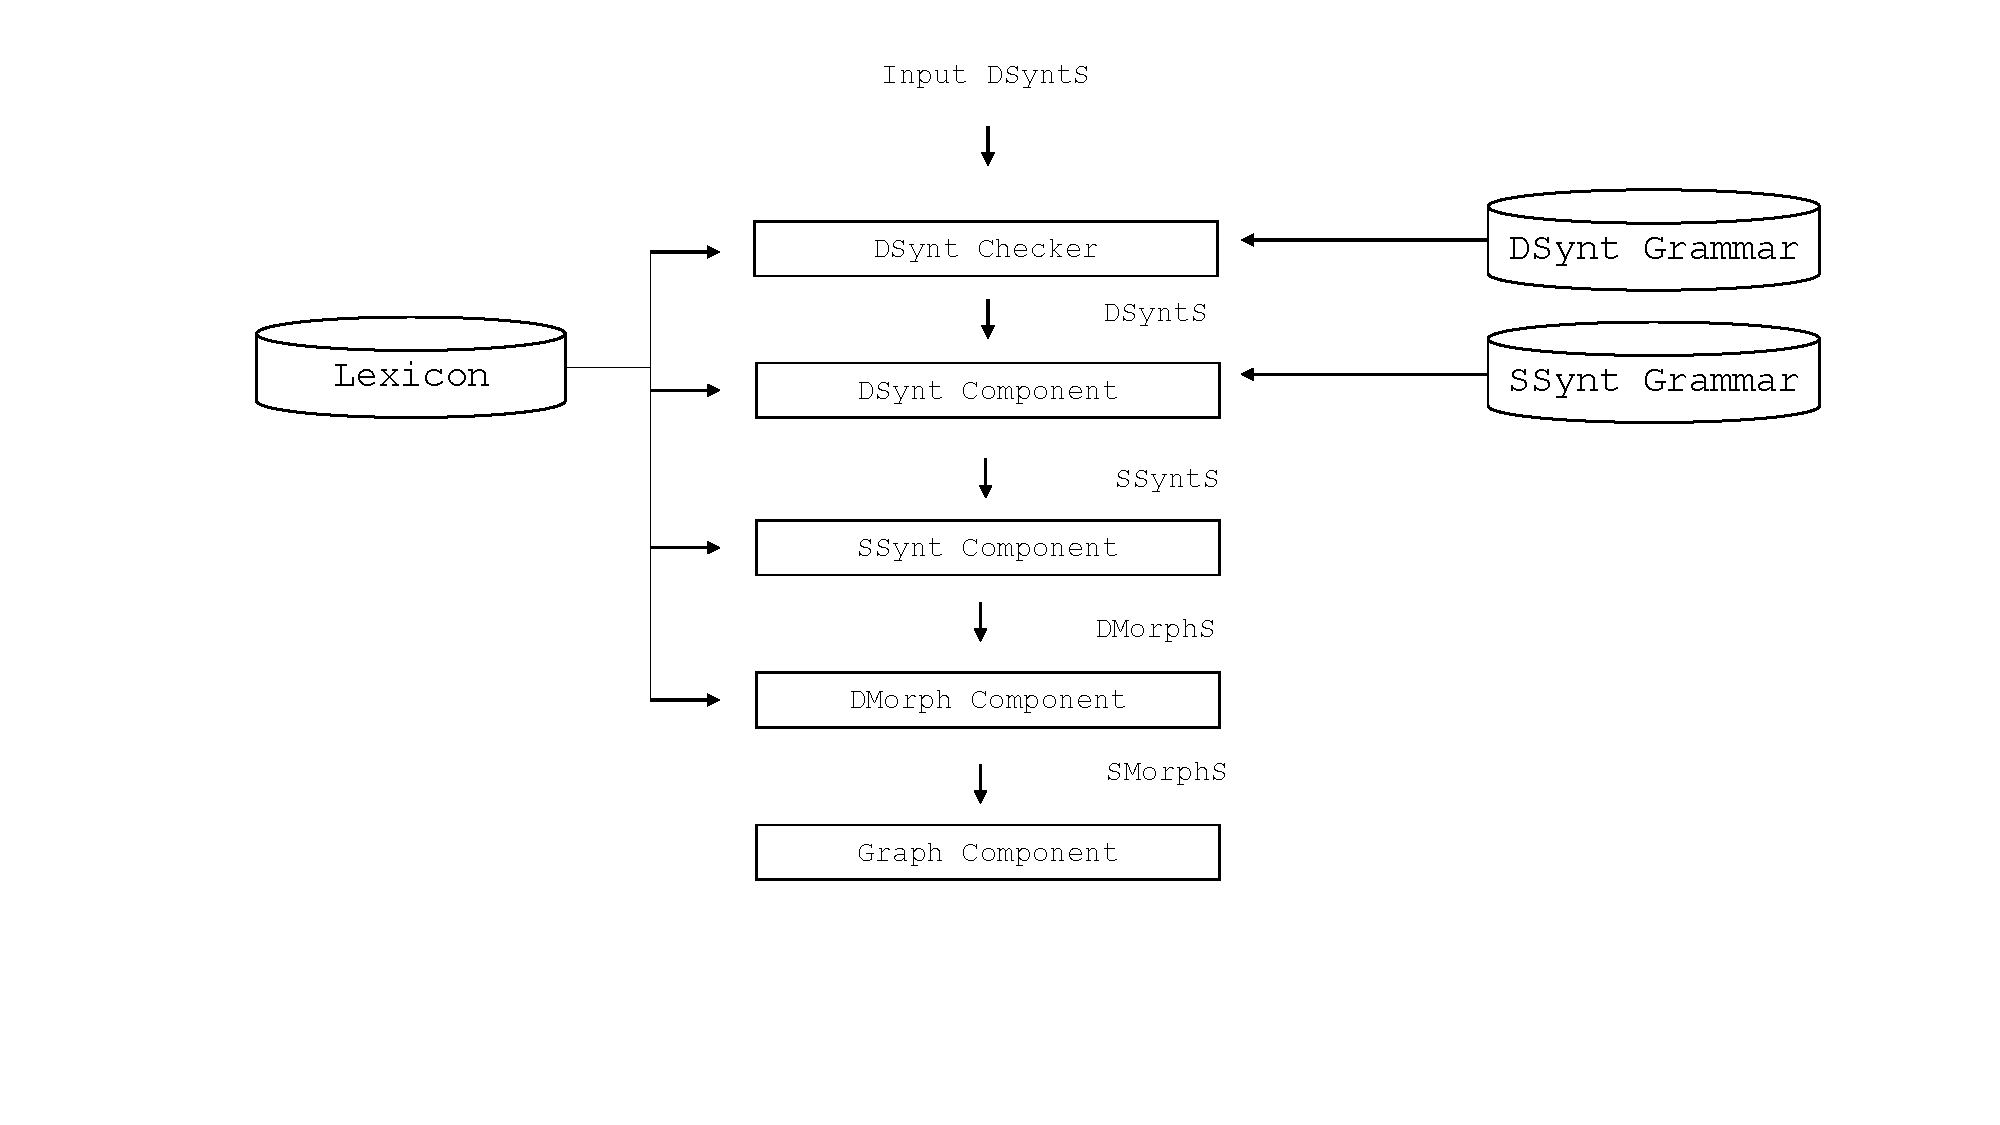
\includegraphics[width=1\textwidth, trim = {0cm 0cm 0cm 0cm},clip]{ch2/figs/realpro.pdf}
	\caption{RealPro}
	\label{fig:RealPro}
\end{figure}

Le dictionnaire contient de l'information quant à la partie du discours et les irrégularités morphologiques pour contourner les règles de grammaires dont celle qui ajoute \emph{-ed} à la fin des verbes au passé. Ainsi, cette information est encodée dans l'entrée de dictionnaire.

\begin{lstlisting}[language=Xml, caption=Entrée de dictionnaire]
LEXEME: SEE
CATEGORY: verb
MORPHOLOGY:[([mood:past-part] seen [inv])
            ([tense:past]     saw  [inv])]
\end{lstlisting}

\draft{je pourrais aussi ajouter la structure de dépendance pour montrer l'input de : This boy sees Mary.}

\subsubsection{KPML}
KMPL\citep{BatemanEnablingTechnologyMultilingual1997} est une extension multilingue du système de PENMAN (citation). C'est un système basé sur la grammaire fonctionnelle systémique (Halliday,1985). KPML contient trois éléments : un engin computationnel qui passe au travers de ressources grammaticales, une collection de ressources grammaticales, un environnement de développement pour écrire et débugger de nouvelles grammaires. Il s'agit d'un système puissant et complexe. Sa grammaire s'appelle NIGEL, il s'agit d'une grammaire de l'anglais. Toutefois, KPML se veut une ressource multilingue et elle couvre aussi des langues comme l'Allemand et le Néerlandais.

KPML prend des SPL en entrée. Il s'agit de \emph{Sentence Planning Language}. Afin d'illustrer à quoi ressemble l'input, nous allons nous servir de Dale et Reiter qui montre une phrase exemple 'March had some rainy days'.
\begin{lstlisting}[language=Xml, caption=SPL: input de KPML]
(S1 \ generalized-possession
  :tense past 
	:domain (N1 \ time-interval
	            :lex march
							:determiner zero)
	:range (N2 \ time-interval
	           :number plural
						 :lex day
						 :determiner some
						 :property ascription
						 (A1 \ quality :lex rainy)))
\end{lstlisting}
Compléter avec Florie

\subsubsection{MARQUIS}
\citep{WannerMARQUISGENERATIONUSERTAILORED2010}

\subsubsection{Forge: héritier de MARQUIS}
\citep{DBLP:conf/semeval/MilleCBW17}

\subsubsection{Surge}
\citep{Elhadad98surge:a}
Surge qui signifie \emph{Systemic Unification Realisation Grammar of English}, c'est une grammaire à grande couverture. Elle est écrite en FUF \emph{Functional Unification Formalism}. Il s'agit d'un langage de programmation créé pour construire des grammaires computationnelles, plus particulièrement pour les besoins de la réalisation linguistique dans un cadre de grammaire d'unification. Est basé sur FUG (Kay,1979) et ils se servent de graphes d'unification comme input à leur système. Cet input est sous forme de FD (Functional Description), il s'agit d'une collection de paires attributs-valeurs dont l'union fournit une spécification de l'énoncé à génerer. Chaque FD contient un trait CAT qui indique la catégorie syntaxique de la forme à produire. Les autres attributs dépendent de l'information requise par la grammaire pour générer une structure de cette catégorie

Par exemple, tel que trouvé dans Dale et Reiter, voici l'exemple d'une structure d'input pour 'March had some rainy days'.
\begin{lstlisting}[language=Xml, caption=FD: input de Surge]
((cat clause)
 (proc ((type possessive)))
 (tense past)
 (partic ((possessor ((cat proper) head ((lex "March"))))
					(possessed ((cat common) head ((lex day)))
											(describer ((lex rainy)))
											(selective yes) (number plural)))))
\end{lstlisting}

Compléter avec Florie

\subsection{Différences entre réalisateur de surface et profond}
Tel que Lambrey dans \citep{LambreyImplementationcollocationspour2017} l'a dit, les réalisateurs de surface sont plus facile à construire que les réalisateurs profonds. Entre autre parce qu'un RS est (à compléter). Tandis qu'un RP nécessite des linguistes pour développer l'application. Ces derniers sont plus complexes ce qui entraîne des coûts au niveau du temps et des ressources. Leur avantage réside dans le fait qu'ils sont dotés d'une profondeur linguistique leur permettant de faire l'analyse de phénomènes langagiers beaucoup plus complexes qu'un RS peut faire. 

Les RP présentés dans cette section encodent sans exception leurs connaissances linguistiques dans des dictionnaires et des grammaires. On remarquera que leurs différences majeures sont directement liées aux théories linguistiques sous-jacentes qu'ils utilisent pour modéliser la langue. Ainsi des réalisateurs comme Surge ou G-TAG (que nous n'avons pas décrit ici), ne possèdent pas de dictionnaires car leur module de règles contient des arbres partiellement lexicalisés. Tandis que MARQUIS, Forge, RealPro et KPML possèdent respectivement un module de règles grammaticales et des dictionnaires. Ce qui rend ces systèmes plus enclin à traiter plusieurs langues en même temps, et ce avec facilité. Un exemple de système qui fonctionne ainsi est GenDR \citep{lareau18}, un réalisateur profond multilingue qui possède respectivement un dictionnaire séparé de sa grammaire. Ainsi, le système peut générer du texte à partir d'un même input sémantique dans plusieurs langues en même temps en faisant appel à des règles de grammaires partagées (certaines règles sont spécifiques à chaque langue) et des dictionnaires propres à chaque langue.

Dans le cadre de ce mémoire, nous allons nous baser sur GenDR, une extension de MARQUIS. GenDR est un projet en cours de développement dirigé par François Lareau à l’Observatoire de linguistique Sens-Texte. Nous entrerons dans les détails au chapitre suivant.